%\section}
\section*{
نگاه سناریو
\LTRfootnote{ Scenario View}
}
در این بخش به دید سناریو‌ی پروژه می‌پردازیم. به این منظور، دو سناریو که کارکرد سیستم را نشان دهند در نظر می‌گیریم. یک نکته‌ی مهم در مورد سناریو‌ها این است که اگرچه طراحی ما مبنی بر استایل
\lr{MVC}
است، در بعضی از بخش‌ها به علت سادگی مفهومی کنترلر، از اشاره به آن صرف‌نظر کرده‌ایم و مستقیما 
\lr{View}
را به 
\lr{Model}
وصل کرده‌ایم. 
\subsection*{سناریو‌ی پرداخت}
در این سناریو، کاربر به صفحه‌ی کاربری خود مراجعه کرده و با اطلاع از میزان اعتبارش، تصمیم به افزایش اعتبار می‌کند.
شکل این سناریو در 
\ref{figscen:1}
آمده است. مراحل سناریو به شرح زیر هستند.
\begin{enumerate}
	\item 
	ابتدا کاربر درخواست دسترسی به صفحه‌ی پروفایل خود را می‌دهد که توسط 
	\lr{Profile View}، گرفته می‌شود.
	\item 
\lr{Profile View}
با دسترسی به مدل کاربر، درخواست کسب اطلاعات مورد نیاز را  می‌دهد.
%\footnote{
%	در واقع بین 
%	\lr{view}
%	و
%	\lr{controller
%}
\item 
\lr{Profile model}
اطلاعات مورد نیاز را به 
\lr{Profile view}
می‌دهد.
\item 
\lr{Profile view}، 
اطلاعات کاربر را به وی نشان می‌دهد.
\item 
کاربر با دسترسی به صفحه‌ی پرداخت، اقدام به افزایش اعتبار خود می‌کند.
\item 
در صورت موفقیت پرداخت، اعتبار کاربر افزایش می‌یابد.
\item 
نتیجه‌ی تراکنش به اطلاع کاربر می‌رسد.
\end{enumerate}
\begin{figure}[H]
	\centering
	\includegraphics[width=\textwidth]{diagrams/payment.pdf}
	\caption{سناریو‌ی پرداخت ‌ }
	\label{figscen:1}	
\end{figure}
\subsection*{سناریو‌ی اجاره}
در این سناریو، کاربر با دسترسی به صفحه‌ی جست‌و‌جو، ابتدا کالای مورد نظر خود را می‌یابد و سپس با بررسی مشخصات آن، اقدام به اجاره می‌کند. شکل این سناریو در 
\ref{figscen:2}
آمده است.
\begin{enumerate}
	\item 
	ابتدا کابر با دسترسی به صفحه‌ی جست‌وجو، لیست کالاهای مورد نظرش را می‌خواهد.
	\item 
	صفحه‌ی جست‌و‌جو لیست کالاهای مناسب را با درخواست دادن به 
	\lr{product model}
	به دست می‌آورد.
	\item 
	لیست مورد نظر به کاربر داده می‌شود.
	\item 
کاربر درخواست مشاهده‌ی مشخصات کالای مورد نظر را می‌دهد.
\item 
اطلاعات کالای مورد نظر تهیه از 
\lr{Product model}
گرفته می‌شود.
\item 
اطلاعات کالا به کاربر نشان داده می‌شود.
\item
کاربر اقدام به ثبت سفارش می‌کند.
\item 
درخواست ثبت سفارش به 
\lr{Order controller}
داده می‌شود.
\item 
اطلاعات کالای مورد نظر از قبیل قابل اجاره بودن و قیمت تهیه می‌شود.
\item 
اطلاعات مالی کاربر با درخواست دادن به 
\lr{Profile model}
تهیه می‌شود.
\item 
در صورتی که سفارش قابل انجام باشد، سفارش مناسب در 
\lr{Order model}
ثبت می‌شود.
\item 
نتیجه‌ی سفارش به 
\lr{Order view}
داده می‌شود.
\item 
نتیجه‌ی سفارش به کاربر نشان داده می‌شود.
\end{enumerate}
\begin{figure}[H]
	\centering
	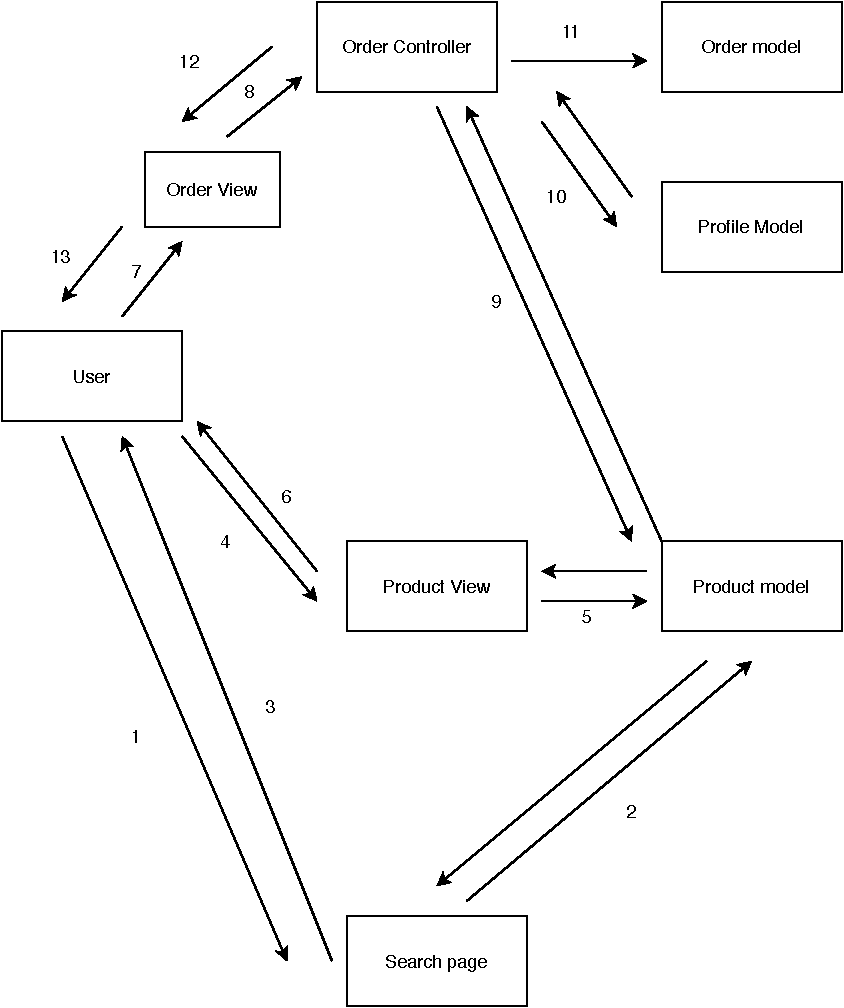
\includegraphics[width=\textwidth]{diagrams/Order.pdf}
	\caption{سناریو‌ی اجاره ‌ }
	\label{figscen:2}	
\end{figure}